\section{Faster Generation of Spanning Trees}

In this section, we will introduce a faster algorithm for generating \emph{approximately uniform} random spanning trees. In particular, we focus on the generation of $\delta-$random spanning trees:

\begin{definition}[$\delta-$random spanning trees]
A randomized algorithm $A$ that generates $\delta-$random spanning trees outputs a random spanning tree $T$ with probability $p(T)$ that is \emph{$\delta-$far from uniform}, i.e., 
$$\frac{1-\delta}{|\mathcal{T}(G)|}\leq p(T) \leq \frac{1+\delta}{|\mathcal{T}(G)|}$$
where $\mathcal{T}(G)$ is the set of spanning trees of $G$.
\end{definition}

% \subsection{$\delta-$random spanning trees and arborescences}

% \subsection{Algorithm}

With the same reasoning as before, if we get a procedure that generates $\delta-$random arborescences, it also gives a procedure that generates $\delta-$random spanning trees. 

\cite{kelner2009faster} introduces a faster generation algorithm which generates $\delta-$random spanning trees in expected time of $\bigotilde(m\sqrt{n}\log(1/\delta))$. For brevity of illustration, we will focus on a simplified algorithm that gives an expected running time of $\bigotilde(m^2/\sqrt{n}\log(1/\delta))$, which shares the same spirit.

%Haonan: Moved to part 1
%Before discussing the algorithm, it will be useful to introduce \emph{arborescences} defined as below:
%\begin{definition}{Arborescence}    
%    For a given $s \in G$, an arborescence $T$ \emph{rooted at $s$} is a directed spanning tree of $G$ where all vertices in $G \setminus \set{s}$ have \emph{exactly one} incoming arc.
%\end{definition}

%It is easy to check that there is a one-to-one correspondence between spanning trees of $G$ and arborescences rooted at $s$: given any spanning tree, there is a unique way of directing its edges to make it an arborescence rooted at $s$; conversely, given any arborescence rooted at $s$, one can obtain a spanning tree by simply disregarding the direction of the edges.
%Therefore, if we get a procedure that generates ($\delta-$random) arborescences, it also gives a procedure that generates ($\delta-$random) spanning trees. 
%In fact, the random walk algorithm simulates the generation of arborescences.

The key idea of the algorithm is the observation that the random walk algorithm may spend a long time walking in regions that have already been covered. Indeed, the random walk algorithm has a running time of $O(mn)$, while only a tiny fraction $O(n)$ is used for recovering an arborescence.
Therefore, the algorithm seeks to obtain a shortcut that cuts out the random walk corresponding to visiting already explored parts of $G$.
The essential steps are to first decompose the graph into small subgraphs that can be quickly covered, and then shortcut the walk inside each subgraph \emph{if it is already covered}.

\subsection{Decompose the graph}
First, we define the $(\phi, \gamma)$-Decomposition that will permit the implementation of the fast generation algorithm. 
Let $(D_1, \dots, D_k, S, C)$ denote a partition of $G$, where $D_i$ are disjoint subgraphs, $S=V(G) \setminus \bigcup_i V(D_i)$ is the set of remaining vertices, and $C=E(G) \setminus \bigcup_i E(D_i)$ is the set of edges not entirely contained inside one of $D_i$. 
For a given $D_i$, let $C(D_i)$ be the subset of $C$ incident to $D_i$ and $U(D_i)$ be the set of vertices of $D_i$ incident to an edge from $C$.

\begin{definition}[$(\phi, \gamma)$-decomposition]
   $(D_1, \dots, D_k, S, C)$ is a $(\phi, \gamma)$-decomposition if:
   \label{def:decomposition}
\begin{enumerate}
    \item $|C| \leq \phi |E(G)|$
    \item $\forall i$, the diameter $\gamma(D_i) \leq \gamma$
    \item $\forall i$, $|C(D_i)| \leq |E(D_i)|$
\end{enumerate}
\end{definition}
Note that the first condition ensures that the subgraphs $D_1, \dots, D_k$ contain most (all but a $\phi$ fraction of) edges in $G$.
Intuitively, the second condition ensures that each subgraph could be covered relatively quickly, using the fact that the cover time of an unweighted graph $G'$ with diameter $\gamma(G')$ is at most $O(|E(G')|\gamma(G'))$ \cite{aleliunas1979random}.

For reasons that will become clear later, we consider a specific decomposition that can be quickly computed, shown by the following lemma:
\begin{lemma}[Obtaining good ($(\phi, \gamma)$-decompositions]
\label{lem:decompose}
For $G$ and any $\phi=o(1)$, a $(\phi, \bigotilde(1/\phi))$-decomposition of $G$ can be computed in time $\bigotilde(m)$.
\end{lemma}
We omit the proof for brevity and refer interested readers to Lemma 13 and its proof in \cite{kelner2009faster}.

\subsection{Decompose the walk}
Then, we considet the random walk $X=(X_i)$  over the decomposed graph started from a vertex chosen by the stationary distribution $G$. 
Let $\tau$ be the cover time of $G$, i.e., the first time that the walk visits all the vertices of $G$.
The result in \cite{aleliunas1979random} yields that $E[\tau]=O(mn)$ which is the expected time of traditional random walk.

We decompose the walk over decomposed $G$.
Let $Z$ and $Z_i$ be the random variables corresponding to the number of times that $X$ traverses edges from $C$ and inside $D_i$ respectively. 
By definition, we have that $\tau=\sum_i Z_i + Z$. The following lemma establishes the expectation of $Z$:
\begin{fact}
    \label{fact:traverse}
    The expected traversed time in $C$ is $E(Z)=O(\phi mn)$. 
\end{fact}
\begin{proof}
    Since the random walk starts from the stationary distribution of $G$, the expected number of traversals of edges from $C$ is just proportional to its size. Therefore, the assumption $|C| \leq \phi |E(G)|$ implies the above fact.
\end{proof}

As discussed before, we will be interested in the cover time for each subgraph. In particular, let $Z^*_i$ be the random variable corresponding to the number of traversals inside $D_i$ until $X$ explores the whole subgraph $D_i$, we have that:
\begin{lemma}[Expected cover time for subgraphs]
    \label{lem:cover}
    $E[Z_i^*] = \bigotilde(|E(D_i)|\gamma(D_i))$.
\end{lemma}
\begin{proof}
Let us fix $D = D_i$. For a vertex $v \in V(D)$, let $d_G(v)$ be the degree of $v$ in $G$ and $d_D(v)$ be the degree of $v$ in $G$. For $u,v \in U(D)$, let $p_{u,v}^D$ be the probability that a random walk in $G$ that starts at $u$ will reach $v$ through a path that does not pass through any edge inside $D$. Consider a (weighted) graph $D'$, which we obtain from $D$ by adding, for each $u,v \in U(D)$, an edge $(u, v)$ with weight $d_G(u) p_{u,v}^D$. We note that if we take our walk $X$ and filter out of the vertices that are not from $D$, then the resulting "filtered" walk $Y_D$ will just be a natural random walk in $D'$. As a result, it is easy to see that, in this case, $E[Z_i^*]$ can be upper-bounded by the expected time needed by a random walk in $D'$, started at arbitrary vertex, to visit all of the vertices in $D'$ and then reach some vertex in $U(D)$. Therefore, to bound $E[Z_i^*]$, it suffices to bound the cover time of $D'$. The cover time of undirected graph $G'$ is at most $2\log|V(G')|H_{max}(G')$, where $H_{max}(G')$ is the maximal hitting time. Following the results of \cite{aleliunas1979random}, we have $H_{max}(G') \leq |E(G')|\gamma(G')$. 
\end{proof}
%\begin{proof}
    %\textcolor{red}{TODO}: Refer to Lemma 6 in \cite{kelner2009faster}.
%\end{proof}

\subsection{Shortcut the walk}
Recall that the key idea of the algorithm is to shortcut the trajectory inside $D_i$ after $D_i$ has already been covered. 
More specifically, consider the walk after $D_i$ is covered, this means that we already know for all edges $v \in V(D_i)$ which arc $e_v$ should be added to the arborescence. 
Any further walk inside $D_i$ provides no new information for constructing the arborescence, and could be shortcutted.

\begin{figure}[t!]
        \centering
        \begin{subfigure}[b]{.35\textwidth}
            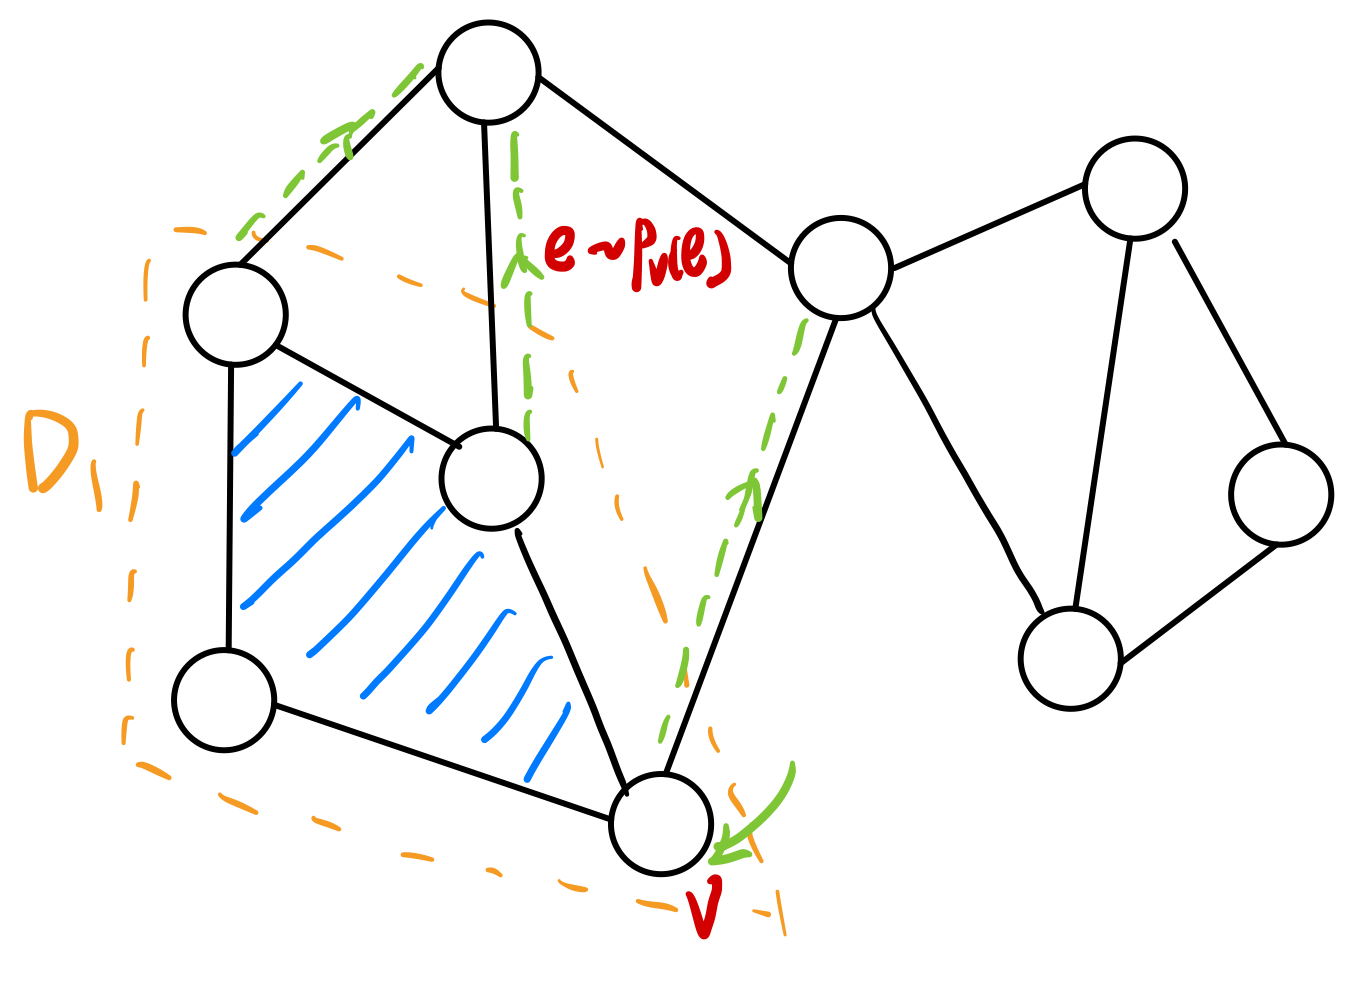
\includegraphics[width=0.9\linewidth, trim={1cm 1cm 1cm 0},clip]{figs/shortcut_impl.jpeg}
            \caption{}
            \label{fig:shortcut_impl}
        \end{subfigure}
        \begin{subfigure}[b]{.62\textwidth}
            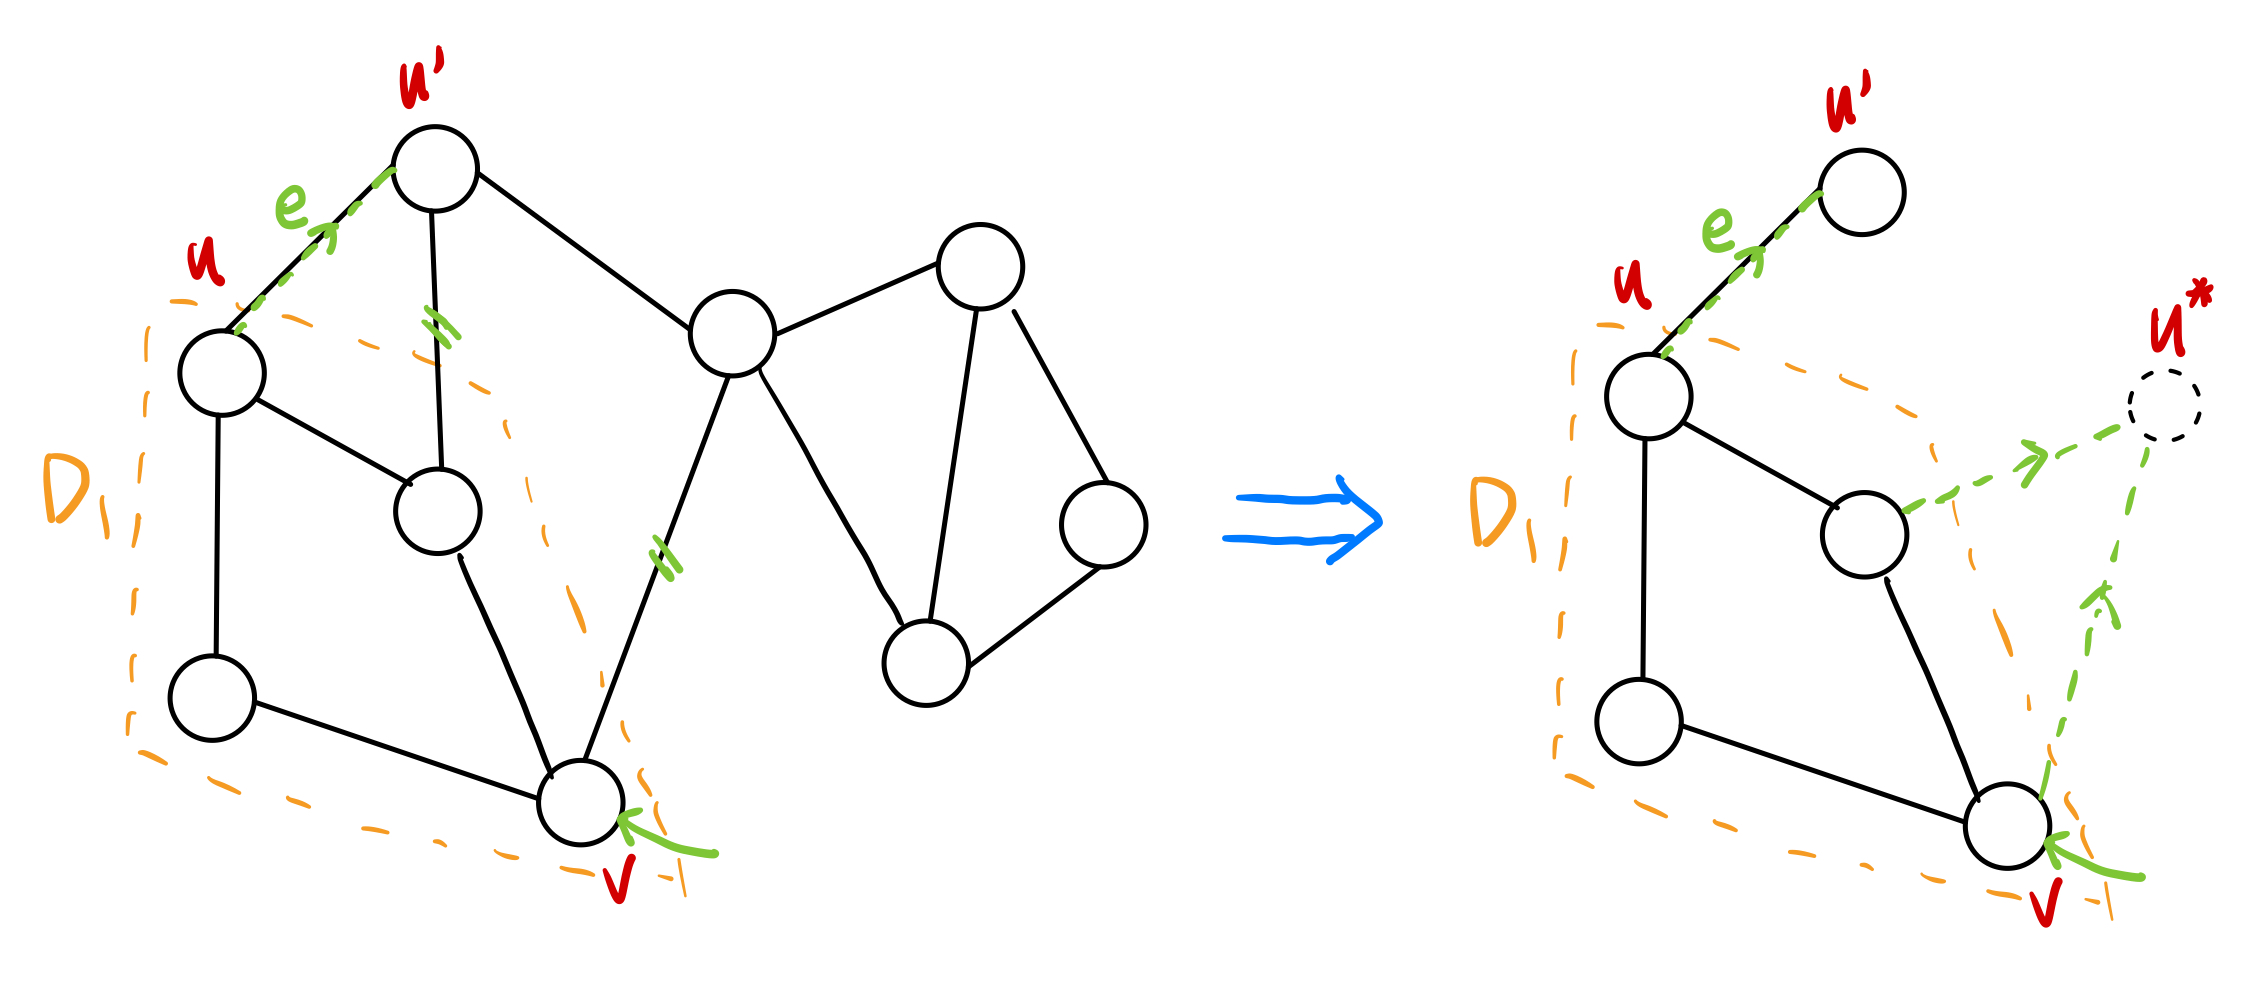
\includegraphics[width=0.95\linewidth, trim={1cm 1cm 1cm 0},clip]{figs/compute_prob.jpeg}
            \caption{}
            \label{fig:compute_prob}
        \end{subfigure}
        \caption{(a) The shortcut of trajectory inside $D_1$ Is implemented by $P_v(e)$ that characterizes the probability of $X$ leaving $D_1$ through edge $e$ after entering through vertex $v$; (b) The illustration for computing $P_v(e)$ by adding a dummy node $u^*$ which connects to all other leaving edges.}
\end{figure}

The main tool for implementing the shortcut is $P_v(e)$ that characterizes the probability of $X$ leaving $D_i$ \emph{through edge $e$ after entering through vertex $v$}, see Fig.\ \ref{fig:shortcut_impl} for an illustration.
If we know $P_v(e)$ for all $v \in V(D_i)$ and all $e \in C(D_i)$, then we could essentially immediately choose the leaving edge $e$ upon entering $v$ without computing the explicit trajectory in $D_i$.

To formalize the intuition, let $\bar{X}=(\Bar{X}_1, \dots, \Bar{X}_m)$ be a decomposition of the walk $X=(X_1, \dots, X_\tau)$ into contiguous blocks $\Bar{X}_j$ that are contained in $D_{i_j}$ for $i_j \in \{0, \dots, k\}$, where $D_0=S$.
We construct the shortcutted walk $\Tilde{X}=(\Tilde{X}_i)$ by processing $\bar{X}$ block by block: 
if $D_{i_j}$ has not been covered or $i_j=0$, we copy $\Bar{X}_j$ to $\Tilde{X}$, otherwise we copy only the first and last entries of the block.

With $P_e(v)$, the following lemma establishes that $\Tilde{X}$ can be simulated efficiently:
\begin{lemma}[Simulating $\tilde{X}$ with $P_v(e)$]
\label{lem:simulate}
        Knowing $P_v(e)$ for all $e \in C(D_i), v \in V(D_i)$ and $i$, we can preprocess these values in $\bigotilde(\phi mn)$ time and it allows simulation of $l$ steps of $\tilde{X}$ in time $\bigotilde(l)$.
\end{lemma}
\begin{proof}
    Simulating $\Tilde{X}$ before $D_i$ is covered is straightforward. The only thing to show is that the shortcutting of blocks can be simulated efficiently. To show this, we consider some $i$ and $v \in U(D_i)$, and construct an array $A_v(m)$ where $A_v(m) = \sum_
{1\leq j \leq m} P_v(e_j)$ for $m \in \{1, \dots, |C(D_i)|\}$ in $\bigotilde(|C(D_i)|)$. So we can construct for all $v \in U(D_i)$ in $\bigotilde(|C(D_i)||V(D_i)|)$. Summing over all $D_i$ gives the above bound on preprocessing time.
Furtheremore, this array enables choosing $e$ with $P_v(e)$ with binary search in polylogarithmic time. 
\end{proof}

From this lemma, we can show that we can find a random arborescence of $G$ efficiently:
\begin{lemma}[Finding a random arborescence]
\label{lem:find_abr}
        Given a $(\phi, \gamma)$-decomposition of $G$ and $P_v(e)$, we can find a random arborescence of $G$ in expected time $\bigotilde(m(\gamma+\phi n))$.
\end{lemma}
\begin{proof}
    We only need to compute the expected length of the shortcutted walk $\Tilde{X}$, which is upper-bounded by the following quantity:
    $$\sum_i \underbrace{E[Z_i^*]}_{\text{cover time of}~D_i} + \underbrace{E[Z]}_{\text{traversals in}~C} + \underbrace{2E[Z]}_{\text{shortcutted traversals }}$$
    The first and the second terms are obvious, and the last term is due to the fact that the two vertices that remain in $\Tilde{X}$ after shortcutting some block from $X$ can be amortized into the number of traversals by $X$ of some edges in $C$.
    By the second assumption in Definition \ref{def:decomposition}, Fact \ref{fact:traverse}, Lemma \ref{lem:cover}, we get that $\sum_i E[Z_i^*] + 3 E[Z] =\bigotilde(\sum_i |E(D_i)\gamma + \phi mn|) = \bigotilde(m(\gamma + \phi n))$. By Lemma \ref{lem:simulate}, the shortcutted work can be simulated in expected time $\bigotilde(m(\gamma + \phi n))$.
\end{proof}

Then the remaining question is whether we can compute $P_e(v)$ efficiently, established by the following lemma:
\begin{lemma}[Computing $P_v(e)$]
    \label{lem:compute_prob}
    Given a $(\phi, \gamma)$-decomposition of $G$, we can compute multiplicative $(1+\varepsilon)$-approximations of $P_v(e)$ in time $\bigotilde(\phi m^2 \log(1/\varepsilon))$
\end{lemma}
\begin{proof}
    Let us fix some $D=D_i$ and an edge $e=(u, u') \in C(D)$ with $u \in U(D)$. Consider a graph $D'$ obtained by adding a dummy node $u^*$ to $D$ and then connecting all other leaving edges to $u^*$, i.e., for each $(w, w') \in C(D) \setminus \{e\}$, we add an edge $(w, u^*)$ (note that $w'$ can be equal to $u'$), see Fig. \ref{fig:compute_prob} for an illustration. Note that $P_v(e)$ is the probability that the walk started at $v$ will \emph{hit $u'$ before $u^*$}, which can be quickly computed using \emph{electrical flows}.

    In particular (see, e.g., \cite{lovasz1993random}), we can treat $D'$ as an electrical circuit where we impose voltage of $1$ at $u'$ and $0$ at $u^*$, then the voltage achieved at $v$ is exactly equal to $P_v(e)$. We can compute a $(1+\varepsilon)$-approximation in $\bigotilde(|E(D')|\log1/\varepsilon)$ using the linear solver in \cite{spielman2014nearly}. Computing for each $e \in C(D)$ and store the probabilities for all vertices $v$, the total running time can be bounded by $\bigotilde(|C|\sum_i |E(D_i)| \log 1/\varepsilon)=\bigotilde(\phi m^2 \log 1/\varepsilon)$, where we use the fact that $|E(D')| = |E(D)| + |C(D)| \leq 2 |E(D)|$ by assumption 3 in Definition \ref{def:decomposition}.
\end{proof}

Note that the above lemma only gives an approximation of $P_v(e)$. We need to show that it is sufficient for controlling the overall error and maintaining a good running time:
\begin{lemma}[An approximate $P_v(e)$ is sufficient]
    \label{lem:sufficiency}
    Given a $(\phi, \gamma)$-decomposition of $G$ and multiplicative $(1+\varepsilon)$-approximation of $P_v(e)$, we can generate a $\delta-$random arborescence of $G$ in expected time $\bigotilde(m^2(\gamma+\phi n))$ as long as $\varepsilon \leq \delta / mn$.
\end{lemma}
%\begin{proof}
We omit the proof for brevity and refer interested readers to Lemma 10 and its proof in \cite{kelner2009faster}.%\cite{kelner2009faster}.    
%\end{proof}


Putting all together, we have the theorem establishing the running time of the algorithm:
\begin{theorem}[Total complexity]
    For any $\delta>0$, we can generation a $\delta-$random spanning tree of $G$ in expected time of $\bigotilde(m/\sqrt{n}\log(1/\delta))$.
\end{theorem}
\begin{proof}
    Let $\phi=1/n^{1/2}, \varepsilon=\delta/mn$, the total expected time can be decomposed as:
    \begin{enumerate}
        \item Get a $(1/n^{1/2}, \bigotilde(n^{1/2}))$-decomposition: $\bigotilde(m)$ (Lemma \ref{lem:decompose}).
        \item Compute estimate of $P_v(e)$: $\bigotilde(m^2/\sqrt{n}\log(1/\delta))$ (Lemma \ref{lem:compute_prob}).
        \item Generate a $\delta$-arborescence: $\bigotilde(m\sqrt{n})$ (Lemma \ref{lem:find_abr}, Lemma \ref{lem:sufficiency}).
    \end{enumerate}
    Summinga all together, we have the total running time of $ \bigotilde(m^2/\sqrt{n}\log(1/\delta))$.
\end{proof}

We refer interested readers to Sec. 4 in \cite{kelner2009faster} for an improved algorithm with $\bigotilde(m\sqrt{n}\log(1/\delta))$, which is obtained by a stronger decomposition and a slightly different random walk.

